\documentclass[conference]{IEEEtran}

\usepackage{amsmath,amssymb}
\usepackage{graphicx}
\usepackage{booktabs}
\usepackage{multirow}
\usepackage{array}
\usepackage{cite}
\usepackage{xcolor}
\usepackage{url}
\usepackage{algorithm}
\usepackage[noend]{algpseudocode}
\usepackage{tikz}
\usetikzlibrary{arrows.meta,positioning,fit}
\usepackage[hidelinks]{hyperref}

\definecolor{auditblue}{HTML}{2A6F97}
\definecolor{auditred}{HTML}{C43C4E}
\definecolor{auditgreen}{HTML}{315B55}
\newcommand{\meanpm}[2]{#1\,$\pm$\,#2}
\newcommand{\protocol}[1]{\textsf{#1}}
\newcommand{\cytofair}{\textsc{CytoFair}}
\newcommand{\placeholder}[1]{\texttt{[#1]}}
\setlength{\textfloatsep}{6pt plus 1pt minus 2pt}
\setlength{\dbltextfloatsep}{6pt plus 1pt minus 2pt}
\setlength{\floatsep}{5pt plus 1pt minus 2pt}
\setlength{\dblfloatsep}{5pt plus 1pt minus 2pt}
\setlength{\abovecaptionskip}{3pt}
\setlength{\belowcaptionskip}{0pt}
\renewcommand{\arraystretch}{0.92}

\title{Do We Train on Test Cells? Provenance Leakage in Public Cervical Cytology Benchmarks}

\author{
\IEEEauthorblockN{Snehasish Ghosh\IEEEauthorrefmark{1},
Soham Mitra\IEEEauthorrefmark{2}, and
Nibaran Das\IEEEauthorrefmark{2}}
\IEEEauthorblockA{\IEEEauthorrefmark{1}Indian Institute of Science, Bengaluru, India\\
Email: snehasishg@iisc.ac.in}
\IEEEauthorblockA{\IEEEauthorrefmark{2}Department of Computer Science and Engineering,
Jadavpur University, Kolkata, India\\
Emails: \placeholder{SOHAM EMAIL}, \placeholder{NIBARAN EMAIL}}
}

\begin{document}
\maketitle

\begin{abstract}
Cervical cancer caused an estimated 660,000 new cases and 350,000 deaths worldwide in 2022, making trustworthy automation for cytology screening a public-health priority~\cite{who2025hpv}.
Existing classifiers attain high crop-level accuracy on public cervical-cell benchmarks but often treat several cells from one microscopic field as independent observations, exposing train and test partitions to shared source fingerprints and, in some cases, identical pixels.
We propose \cytofair, a provenance-recovery and grouped-evaluation framework that independently reconstructs crop-to-parent mappings, validates geometry, quantifies structural and literal overlap, tests parent identifiability, and releases fixed parent-disjoint splits.
On SIPaKMeD, parent identification reaches \meanpm{25.73}{0.66}\% versus \meanpm{0.17}{0.24}\% for the label-shuffled comparator, while \meanpm{92.62}{0.40}\% of random-split test crops have a training parent and \meanpm{52.62}{1.97}\% share literal pixels; all six architecture-wise \protocol{P1}$-$\protocol{P2} point estimates are positive, although none survives the preregistered Benjamini--Hochberg correction.
Code, provenance maps, and fixed splits are available at \placeholder{REPOSITORY URL}.
\end{abstract}

\begin{IEEEkeywords}
cervical cytology, data leakage, provenance, grouped splitting, benchmark audit, reproducibility
\end{IEEEkeywords}

\section{Introduction}
Cervical cytology is a high-volume screening task in which a small number of abnormal cells must be recognized among many visually plausible normal cells.
The public-health burden is substantial: cervical cancer was the fourth leading cause of cancer incidence and mortality among women worldwide in 2022~\cite{who2025hpv}.
Computer-assisted screening is therefore attractive not merely as a leaderboard problem, but as a way to support scarce expert attention.
That promise depends on an elementary validity condition: the held-out sample should represent genuinely unseen biological or acquisition units.
The image presented to a network, however, is not always the independent unit sampled from the population.
When several released cell crops originate from one field, they inherit stain, illumination, focus, background texture, preparation artifacts, and sometimes overlapping pixels.
A crop-level split can then put siblings on both sides of evaluation while appearing formally disjoint at the filename level.

Deep learning has substantially advanced cervical-cell analysis.
DeepPap classified cells directly from images and reported 98.3\% accuracy on Herlev~\cite{zhang2017deeppap}; DeepCervix fused features from multiple networks and reported 99.14\% five-class accuracy on SIPaKMeD~\cite{rahaman2021deepcervix}; and a knowledge-distillation framework reported 98.52\% on the same five-class task~\cite{gao2022knowledge}.
These methods draw on residual, dense, efficient, mobile, and transformer backbones whose general image-recognition capabilities are well established~\cite{he2016resnet,huang2017densenet,sandler2018mobilenetv2,tan2019efficientnet,dosovitskiy2021vit}.
Public resources have made such comparisons possible: SIPaKMeD provides 4,049 cell crops derived from 966 cluster fields~\cite{plissiti2018sipakmed}, Cx22 provides 1,320 generated regions with instance labels~\cite{liu2022cx22}, CRIC provides 11,534 classified cells in 400 source images~\cite{rezende2021cric}, and Herlev provides 917 single-cell images~\cite{jantzen2005pap}.
Yet performance engineering has advanced faster than auditing of the sampling hierarchy beneath these released observations.

Establishing defensible benchmark generalization is \emph{challenging} for three concrete reasons.
First, cervical classes can be morphologically similar, making small changes in test composition consequential.
Second, public datasets are small and can be balanced by crop count while remaining highly imbalanced by source-parent count.
Third, parent identifiers are not always carried into downstream crop folders, so ordinary stratified splitting silently discards the hierarchy that generated the data.
The third difficulty is the focus of this work: we recover that hierarchy exactly where the release permits it, measure what crop splitting shares, and construct partitions that keep a parent---and, in a conservative sensitivity analysis, a near-duplicate component---wholly in one arm.
We distinguish structural non-independence from causal classifier use: recoverable parent information shows that a shortcut is available, not that every class model necessarily uses it.

Our contributions are exactly fourfold:
\begin{itemize}
    \item \cytofair, an auditable framework for exact crop-to-parent recovery, deterministic validation, and provenance-aware split generation;
    \item the first complete dual-branch provenance map for all 4,049 SIPaKMeD crops, together with source recovery for Cx22 and structural audits of CRIC and Herlev;
    \item direct measurements of random-split parent straddling, literal cross-split pixel sharing, and a five-seed parent-identity probe with transformation and shuffled-label controls;
    \item extensive experiments on SIPaKMeD, Cx22, CRIC, and Herlev demonstrate that crop-level evaluation can be structurally non-independent and that fixed parent-disjoint splits remove the measured sharing.
\end{itemize}

\section{Related Work}
\subsection{Cervical Cell Classification}
Zhang \emph{et al.} proposed DeepPap, achieving 98.3\% accuracy on the Herlev benchmark; however, cervical crop-to-parent provenance was outside its scope~\cite{zhang2017deeppap}.
Rahaman \emph{et al.} proposed DeepCervix, achieving 99.14\% five-class accuracy on SIPaKMeD; however, cervical crop-to-parent provenance was outside its scope~\cite{rahaman2021deepcervix}.
Gao \emph{et al.} proposed a transfer-learning and knowledge-distillation classifier, achieving 98.52\% five-class accuracy on SIPaKMeD; however, cervical crop-to-parent provenance was outside its scope~\cite{gao2022knowledge}.
These numbers establish the maturity of crop classification, but they are not imported into our comparison because nominally identical datasets under different splits do not define comparable tests.

\subsection{Leakage, Duplicates, and Identity}
Barz and Denzler proposed ciFAIR, identifying training counterparts for 3.3\% and 10\% of CIFAR-10 and CIFAR-100 test images; however, cervical crop-to-parent provenance was outside its scope~\cite{barz2020cifair}.
Laroca \emph{et al.} proposed duplicate-free license-plate splits, re-evaluating six recognition models on AOLP and CCPD; however, cervical crop-to-parent provenance was outside its scope~\cite{laroca2023lpr}.
Packh\"auser \emph{et al.} proposed a chest-radiograph re-identification system, achieving 95.55\% identity accuracy on ChestX-ray14; however, cervical crop-to-parent provenance was outside its scope~\cite{packhauser2022reidentification}.
Kapoor and Narayanan situated non-independence within a broader taxonomy of leakage and scientific reproducibility failures~\cite{kapoor2023leakage}.
Table~\ref{tab:prior} makes the shared scope boundary explicit without labeling any individual study deficient.
The gap remains an exact, validated provenance audit and corrected public evaluation resource for cervical-cytology crop benchmarks; this paper addresses it.

\begin{table*}[t]
\caption{Representative prior work and the common scope gap.}
\label{tab:prior}
\centering
\scriptsize
\setlength{\tabcolsep}{8pt}
\begin{tabular}{llll}
\toprule
Work & Method / audit & Reported result & Limitations relative to this study \\
\midrule
DeepPap~\cite{zhang2017deeppap} & Direct CNN & 98.3\% Herlev & Cervical parent provenance not studied \\
DeepCervix~\cite{rahaman2021deepcervix} & Feature fusion & 99.14\% SIPaKMeD & Cervical parent provenance not studied \\
Gao \emph{et al.}~\cite{gao2022knowledge} & Distillation & 98.52\% SIPaKMeD & Cervical parent provenance not studied \\
ciFAIR~\cite{barz2020cifair} & Duplicate audit & 3.3/10\% test duplicates & Cervical parent provenance not studied \\
Laroca \emph{et al.}~\cite{laroca2023lpr} & Fair LPR splits & Six models & Cervical parent provenance not studied \\
Packh\"auser \emph{et al.}~\cite{packhauser2022reidentification} & Identity probe & 95.55\% ChestX-ray14 & Cervical parent provenance not studied \\
\bottomrule
\end{tabular}
\end{table*}

\section{Method}
Figure~\ref{fig:pipeline} summarizes the full pipeline.
\cytofair treats provenance recovery as a prerequisite, not a post-hoc clustering step: released or exactly reconstructed parent identity defines the independent grouping unit, while image-derived similarity is reserved for a separately labeled sensitivity protocol.

\begin{figure*}[t]
\centering
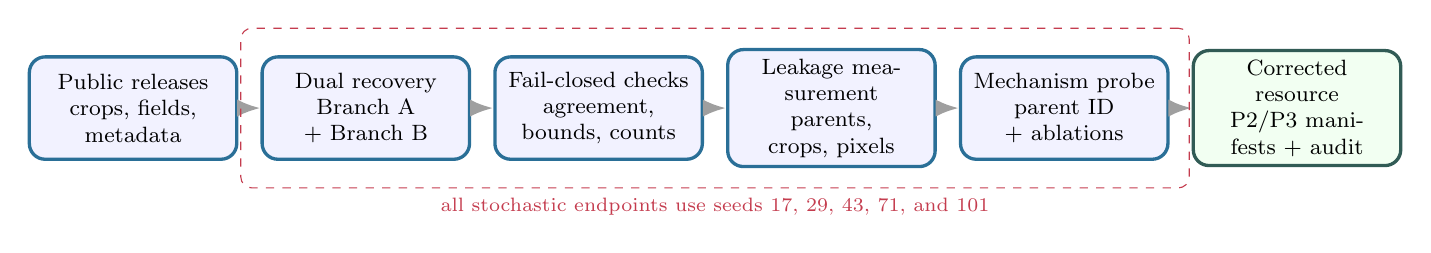
\begin{tikzpicture}[
    node distance=2.8mm,
    >=Latex,
    stage/.style={draw=auditblue, very thick, rounded corners=2mm, fill=blue!5,
                  minimum height=13mm, text width=24mm, align=center, font=\footnotesize},
    result/.style={draw=auditgreen, very thick, rounded corners=2mm, fill=green!5,
                  minimum height=13mm, text width=24mm, align=center, font=\footnotesize},
    arrow/.style={->, very thick, draw=gray!75}
]
\node[stage] (release) {Public releases\\crops, fields, metadata};
\node[stage, right=of release] (recover) {Dual recovery\\Branch A + Branch B};
\node[stage, right=of recover] (validate) {Fail-closed checks\\agreement, bounds, counts};
\node[stage, right=of validate] (measure) {Leakage measurement\\parents, crops, pixels};
\node[stage, right=of measure] (probe) {Mechanism probe\\parent ID + ablations};
\node[result, right=of probe] (release2) {Corrected resource\\P2/P3 manifests + audit};
\draw[arrow] (release) -- (recover);
\draw[arrow] (recover) -- (validate);
\draw[arrow] (validate) -- (measure);
\draw[arrow] (measure) -- (probe);
\draw[arrow] (probe) -- (release2);
\node[draw=auditred, dashed, rounded corners, fit=(recover)(validate)(measure)(probe), inner sep=2.5mm,
      label={[font=\scriptsize,text=auditred]below:all stochastic endpoints use seeds 17, 29, 43, 71, and 101}] {};
\end{tikzpicture}
\caption{The \cytofair{} pipeline. Exact provenance gates every downstream measurement; similarity-derived components affect only the conservative \protocol{P3} sensitivity split.}
\label{fig:pipeline}
\end{figure*}

\subsection{Exact Provenance Recovery}
For each released crop $x_i$, let $g(x_i)=p_j$ denote its source parent.
SIPaKMeD Branch A parses the released filename hierarchy, whereas Branch B ignores that assignment, searches all same-class parent fields, and selects the contained region with maximum normalized cross-correlation
\begin{equation}
\operatorname{NCC}(x,r)=
\frac{\sum_u(x_u-\bar{x})(r_u-\bar{r})}
{\sqrt{\sum_u(x_u-\bar{x})^2\sum_u(r_u-\bar{r})^2}}.
\label{eq:ncc}
\end{equation}
Recovery is accepted only if the branches agree on at least 99\% of common crops, every bounding box lies inside its parent, every crop has exactly one parent, crop totals equal the release, and the reconstructed class-parent counts equal the published vector.
Cx22 parents and requested regions are decoded from the authors' MATLAB generator metadata and checked against the 686-image CCEDD source release; CRIC parent identities come from its released classifications table; one Herlev crop is defined as one parent.

\subsection{Structural and Literal Sharing}
For a parent with $k$ crops assigned independently to 80\% training and 20\% test, the probability of straddling both arms is
\begin{equation}
P_{\mathrm{straddle}}(k)=1-0.8^k-0.2^k.
\label{eq:straddle}
\end{equation}
The analytic dataset expectation is the mean of~\eqref{eq:straddle} over parents.
For an allocation with training-parent set $G_{\mathrm{tr}}$ and test crops $T$, we measure
\begin{equation}
L_{p}=\frac{|G_{\mathrm{tr}}\cap G_{\mathrm{te}}|}{|G|},\quad
L_{c}=\frac{1}{|T|}\sum_{x\in T}\mathbb{1}[g(x)\in G_{\mathrm{tr}}].
\label{eq:leakage}
\end{equation}
For SIPaKMeD, the recovered bounding boxes additionally permit literal sharing: $L_{\mathrm{pix}}$ is the fraction of test crops whose parent has at least one training crop with nonempty source-coordinate intersection.
Observed five-seed estimates are checked against an exact 10,000-allocation Monte Carlo interval under the implemented fixed-size, class-stratified rule.

\subsection{Parent-Identity Mechanism Probe}
Parents with at least four crops enter a balanced closed-set task; each eligible parent contributes the same number of training and test crops.
A ResNet-18 $f_\theta$ is trained with cross-entropy over parent labels,
\begin{equation}
\mathcal{L}_{\mathrm{ID}}(\theta)=-\frac{1}{n}\sum_{i=1}^{n}
\log \frac{\exp f_\theta(x_i)_{g(x_i)}}{\sum_{p}\exp f_\theta(x_i)_p}.
\label{eq:probe}
\end{equation}
The mechanism test asks whether two different crops from one field retain a learnable common fingerprint after cellular content changes; a held-out accuracy of \meanpm{25.73}{0.66}\% shows that the released crop alone contains strongly recoverable parent information.
This establishes availability of a shortcut, not causal use by the downstream class classifier.
The borrowed image transformations isolate candidate substrates: grayscale removes hue, channel-statistics matching follows Reinhard \emph{et al.}~\cite{reinhard2001color}, background-only masks use Otsu thresholds~\cite{otsu1979threshold} followed by Telea inpainting~\cite{telea2004inpainting}, and high-pass filtering suppresses low-frequency illumination.
The same images, optimizer, epochs, and seeds are retained for a parent-label-shuffled control.

\subsection{Matched Evaluation Protocols}
\protocol{P1} is an 80:20 class-stratified crop split.
\protocol{P2} assigns complete recovered parents to one arm.
\protocol{P3} first joins parents connected by cross-parent candidates satisfying both 64-bit pHash and dHash Hamming thresholds of six, then groups the entire connected component; it is a sensitivity analysis, not a claim that every candidate is a proven duplicate.
\protocol{P1$'$} retains the \protocol{P1} test set and, where required, downsamples only its training arm to the exact \protocol{P2} training count.
On SIPaKMeD the counts are already identical, so \protocol{P1$'$}=\protocol{P1}; both preregistered contrasts remain in the multiplicity family for protocol fidelity and are not independent corroboration.

\begin{algorithm}[t]
\caption{Fail-closed provenance-aware evaluation}
\label{alg:cytofair}
\begin{algorithmic}[1]
\Require Released observations $X$, source fields $S$, seeds $\mathcal{R}$
\State Recover $g_A:X\!\to\!S$ from released identifiers
\State Recover $g_B:X\!\to\!S$ by independent content matching
\If{agreement, containment, uniqueness, or count gates fail}
    \State \textbf{stop} and emit an audit ledger
\EndIf
\ForAll{$r\in\mathcal{R}$}
    \State Build \protocol{P1}, \protocol{P1$'$}, \protocol{P2}, and \protocol{P3}
    \State Measure $L_p$, $L_c$, and, when boxes exist, $L_{\mathrm{pix}}$
    \State Train the fixed probe and classifier matrix
\EndFor
\State Report mean $\pm$ sample SD, paired effects, and adjusted inference
\State Export provenance, split hashes, raw runs, and one-command Table-I build
\end{algorithmic}
\end{algorithm}

\subsection{Backbones and Confirmatory Statistics}
The borrowed classifier component comprises ImageNet-pretrained ResNet-18/50~\cite{he2016resnet}, DenseNet-121~\cite{huang2017densenet}, MobileNet-V2~\cite{sandler2018mobilenetv2}, EfficientNet-B0~\cite{tan2019efficientnet}, and ViT-B/16~\cite{dosovitskiy2021vit}; only their final heads are replaced.
For each architecture we pair identical seeds across protocols.
Normal paired differences receive a two-sided paired $t$-test and Cohen's $d_z$; otherwise the preregistered fallback is Wilcoxon with rank-biserial correlation.
All \protocol{P1}$-$\protocol{P2} and \protocol{P1$'$}$-$\protocol{P2} classifier tests form one 12-test Benjamini--Hochberg family~\cite{benjamini1995fdr}; effect-size intervals use 10,000 paired bootstrap resamples.

\section{Experiments}
\subsection{Datasets and Integrity Checks}
Table~\ref{tab:classes} gives the independently reconstructed SIPaKMeD class counts and one representative class-stratified \protocol{P1} allocation.
The 4,049 crops map to 966 parents, Cx22's 1,320 generated regions map to 514 recovered CCEDD sources, CRIC's 11,534 labeled cells map to 400 images, and Herlev contains 917 one-crop parents~\cite{plissiti2018sipakmed,liu2022cx22,rezende2021cric,jantzen2005pap}.
Branch A and Branch B agree on 4,049/4,049 SIPaKMeD crops, all recovered boxes are contained, and the class-parent vector is 126/108/238/271/223.
No observation is excluded.

\begin{table}[t]
\caption{SIPaKMeD counts and \protocol{P1} seed-17 split. Counts are deterministic.}
\label{tab:classes}
\centering
\scriptsize
\setlength{\tabcolsep}{4.0pt}
\begin{tabular}{lrrrr}
\toprule
Class & Crops & Parents & Train & Test \\
\midrule
Superficial--Intermediate & 831 & 126 & 665 & 166 \\
Parabasal & 787 & 108 & 630 & 157 \\
Koilocytotic & 825 & 238 & 660 & 165 \\
Metaplastic & 793 & 271 & 634 & 159 \\
Dyskeratotic & 813 & 223 & 650 & 163 \\
\midrule
Total & 4,049 & 966 & 3,239 & 810 \\
\bottomrule
\end{tabular}
\end{table}

\subsection{Implementation Details}
Every stochastic cell uses seeds 17, 29, 43, 71, and 101 and is reported as mean $\pm$ sample SD.
Table~\ref{tab:hparams} records the complete training configuration.
Training used deterministic CUDA kernels where available and at most three NVIDIA RTX A6000 GPUs concurrently; each individual run used one GPU.

\begin{table}[t]
\caption{Fixed hyperparameters for the frozen experiment.}
\label{tab:hparams}
\centering
\scriptsize
\setlength{\tabcolsep}{3.5pt}
\begin{tabular}{lll}
\toprule
Setting & Cell classifier & Parent probe \\
\midrule
Optimizer & AdamW & AdamW \\
Learning rate & $10^{-4}$ & $10^{-4}$ \\
Weight decay & $10^{-4}$ & $10^{-4}$ \\
Batch size & 64 & 64 \\
Epochs & 20 & 15 \\
Input & $224\times224$ RGB & $224\times224$ \\
Augmentation & resized crop, H/V flip & resized crop, H/V flip \\
Initialization & ImageNet pretrained & ImageNet pretrained \\
Seeds & \multicolumn{2}{c}{17, 29, 43, 71, 101} \\
Hardware & \multicolumn{2}{c}{NVIDIA RTX A6000; $\leq$3 concurrent GPUs} \\
Software & \multicolumn{2}{c}{PyTorch 2.9.0, torchvision 0.24.0, CUDA 12.8} \\
\bottomrule
\end{tabular}
\end{table}

\subsection{Metrics}
For $N$ test crops and $C$ classes, with true label $y_i$ and prediction $\hat y_i$, we report
\begin{align}
\mathrm{Acc}&=\frac{1}{N}\sum_{i=1}^{N}\mathbb{1}[y_i=\hat y_i],\\
\mathrm{MacroF1}&=\frac{1}{C}\sum_{c=1}^{C}\frac{2P_cR_c}{P_c+R_c},\\
\mathrm{BAcc}&=\frac{1}{C}\sum_{c=1}^{C}\frac{TP_c}{TP_c+FN_c}.
\end{align}
Accuracy is the preregistered primary endpoint; macro-F1 and balanced accuracy are retained concordance metrics.
Structural endpoints are $L_p$, $L_c$, and $L_{\mathrm{pix}}$ from~\eqref{eq:leakage}.

\subsection{Main Comparison}
Table~\ref{tab:structural} is the central comparison.
The observed straddle means fall inside their exact 10,000-allocation 95\% intervals for all four datasets.
SIPaKMeD has \meanpm{45.63}{1.04}\% straddled parents and \meanpm{92.62}{0.40}\% of test crops with a training parent; Cx22 has \meanpm{34.01}{1.10}\% and \meanpm{85.23}{3.51}\%; CRIC reaches \meanpm{94.35}{1.10}\% and \meanpm{99.97}{0.08}\%.
Herlev, the structural negative control, remains exactly \meanpm{0.00}{0.00}\%.
Both grouped protocols eliminate measured parent sharing.
Among 13,064 within-parent SIPaKMeD crop pairs, 2,185 overlap; under \protocol{P1}, \meanpm{52.62}{1.97}\% of test crops share literal source pixels with a training crop, versus \meanpm{0.00}{0.00}\% under \protocol{P2}/\protocol{P3}.

\begin{table*}[t]
\caption{Structural leakage under crop-level and grouped protocols. Stochastic entries are mean $\pm$ sample SD over five fixed seeds.}
\label{tab:structural}
\centering
\scriptsize
\setlength{\tabcolsep}{5.2pt}
\begin{tabular}{lrrrrrrr}
\toprule
Dataset & Crops & Parents & Analytic \protocol{P1} straddle & Observed \protocol{P1} straddle & \protocol{P1} test crop with train parent & \protocol{P2} straddle & \protocol{P3} straddle \\
\midrule
SIPaKMeD & 4,049 & 966 & 44.83\% & \meanpm{45.63}{1.04}\% & \meanpm{92.62}{0.40}\% & \meanpm{0.00}{0.00}\% & \meanpm{0.00}{0.00}\% \\
Cx22 & 1,320 & 514 & 33.93\% & \meanpm{34.01}{1.10}\% & \meanpm{85.23}{3.51}\% & \meanpm{0.00}{0.00}\% & \meanpm{0.00}{0.00}\% \\
CRIC & 11,534 & 400 & 94.88\% & \meanpm{94.35}{1.10}\% & \meanpm{99.97}{0.08}\% & \meanpm{0.00}{0.00}\% & \meanpm{0.00}{0.00}\% \\
Herlev & 917 & 917 & 0.00\% & \meanpm{0.00}{0.00}\% & \meanpm{0.00}{0.00}\% & \meanpm{0.00}{0.00}\% & \meanpm{0.00}{0.00}\% \\
\bottomrule
\end{tabular}
\end{table*}

Table~\ref{tab:classification} compares all six architectures under identical training settings and split sizes; the corrected \cytofair{} \protocol{P2} column is bold.
Every \protocol{P1}$-$\protocol{P2} point estimate is positive, ranging from \meanpm{0.72}{0.83} to \meanpm{2.25}{1.63} percentage points, but protocol sensitivity is not monotone for every model.

\begin{table*}[t]
\caption{SIPaKMeD test accuracy. All models were rerun in this study under the same 3,239/810 train/test counts. Mean $\pm$ sample SD over five seeds.}
\label{tab:classification}
\centering
\scriptsize
\setlength{\tabcolsep}{7pt}
\begin{tabular}{lrrrr}
\toprule
Architecture & \protocol{P1} crop & \protocol{P1$'$} size-matched & \textbf{\cytofair{} \protocol{P2} parent-disjoint} & \protocol{P3} component-disjoint \\
\midrule
DenseNet-121 & \meanpm{98.12}{0.28}\% & \meanpm{98.12}{0.28}\% & \textbf{\meanpm{96.72}{0.69}\%} & \meanpm{97.38}{0.50}\% \\
EfficientNet-B0 & \meanpm{97.78}{0.49}\% & \meanpm{97.78}{0.49}\% & \textbf{\meanpm{96.69}{1.49}\%} & \meanpm{97.41}{0.71}\% \\
MobileNet-V2 & \meanpm{97.41}{0.45}\% & \meanpm{97.41}{0.45}\% & \textbf{\meanpm{95.16}{1.50}\%} & \meanpm{96.20}{0.93}\% \\
ResNet-18 & \meanpm{97.19}{0.59}\% & \meanpm{97.19}{0.59}\% & \textbf{\meanpm{96.00}{0.89}\%} & \meanpm{96.35}{1.28}\% \\
ResNet-50 & \meanpm{97.51}{0.47}\% & \meanpm{97.51}{0.47}\% & \textbf{\meanpm{96.79}{0.42}\%} & \meanpm{96.27}{0.53}\% \\
ViT-B/16 & \meanpm{97.14}{0.95}\% & \meanpm{97.14}{0.95}\% & \textbf{\meanpm{95.56}{0.84}\%} & \meanpm{95.53}{1.68}\% \\
\bottomrule
\end{tabular}
\end{table*}

\subsection{Mechanism Ablation}
The probe ablation in Table~\ref{tab:probe} shows that parent information persists after every prespecified transformation.
Background-only accuracy is \meanpm{18.68}{1.25}\%, so the signal is not confined to cellular morphology; persistence elsewhere does not identify a single exclusive substrate.
The label-shuffled run is \meanpm{0.17}{0.24}\%, with a five-seed 95\% interval of $-0.14$\% to $0.47$\% that covers the exact 0.2358\% chance baseline.

\begin{table}[t]
\caption{Parent-ID probe ablation on the balanced 424-way task.}
\label{tab:probe}
\centering
\scriptsize
\setlength{\tabcolsep}{4.2pt}
\begin{tabular}{lrr}
\toprule
Input condition & Accuracy & Multiple of chance \\
\midrule
RGB & \meanpm{25.73}{0.66}\% & 109.1$\times$ \\
Grayscale & \meanpm{13.80}{1.12}\% & 58.5$\times$ \\
Stain-normalized & \meanpm{17.31}{0.64}\% & 73.4$\times$ \\
Background only & \meanpm{18.68}{1.25}\% & 79.2$\times$ \\
High-pass & \meanpm{16.27}{0.60}\% & 69.0$\times$ \\
Shuffled labels & \meanpm{0.17}{0.24}\% & 0.7$\times$ \\
\bottomrule
\end{tabular}
\end{table}

\subsection{Significance and Registered Predictions}
Table~\ref{tab:inference} reports every primary \protocol{P1}$-$\protocol{P2} test with its paired effect.
The identical six \protocol{P1$'$}$-$\protocol{P2} rows are retained in the registered 12-test family, rather than presented as independent evidence.
No contrast survives correction; the smallest adjusted value is $q=0.1109$.
Accordingly, the classifier experiment estimates direction and scale of protocol sensitivity, not a confirmatory universal inflation effect.
Architecture ordering also changes: Kendall's $\tau=0.467$ (seed-bootstrap 95\% CI 0.071--0.733, unadjusted $p=0.2722$), with 4/15 pairwise reversals.

\begin{table*}[t]
\caption{Preregistered paired \protocol{P1}$-$\protocol{P2} inference. $\Delta$ is percentage points, $d_z$ is paired Cohen's effect, and $q$ is BH-adjusted over the declared 12-test family.}
\label{tab:inference}
\centering
\scriptsize
\setlength{\tabcolsep}{7.0pt}
\begin{tabular}{lrrrrr}
\toprule
Architecture & $\Delta$, mean $\pm$ SD & Raw $p$ & BH $q$ & Cohen's $d_z$ & Bootstrap 95\% CI for $d_z$ \\
\midrule
DenseNet-121 & \meanpm{1.41}{0.90} & 0.0251 & 0.1109 & 1.561 & [0.985, 4.747] \\
EfficientNet-B0 & \meanpm{1.09}{1.85} & 0.2591 & 0.2591 & 0.588 & [$-0.316$, 4.668] \\
MobileNet-V2 & \meanpm{2.25}{1.63} & 0.0370 & 0.1109 & 1.377 & [0.809, 6.686] \\
ResNet-18 & \meanpm{1.19}{1.28} & 0.1081 & 0.1511 & 0.922 & [0.442, 2.365] \\
ResNet-50 & \meanpm{0.72}{0.83} & 0.1260 & 0.1511 & 0.863 & [0.085, 4.025] \\
ViT-B/16 & \meanpm{1.58}{1.70} & 0.1059 & 0.1511 & 0.931 & [0.057, 4.950] \\
\bottomrule
\end{tabular}
\end{table*}

The registered monotonic accuracy hypothesis is not supported: \protocol{P3} exceeds \protocol{P2} in four of six architecture means (Table~\ref{tab:ordering}).
This failure is retained rather than repaired.
Because \protocol{P3} changes grouped test composition, stronger structural conservatism does not imply monotonically lower finite-sample accuracy.

\begin{table}[t]
\caption{Registered protocol-ordering diagnostic. This is not a class confusion matrix.}
\label{tab:ordering}
\centering
\scriptsize
\begin{tabular}{lc}
\toprule
Architecture & \protocol{P3}$\leq$\protocol{P2}$\leq$\protocol{P1} \\
\midrule
DenseNet-121 & Not supported \\
EfficientNet-B0 & Not supported \\
MobileNet-V2 & Not supported \\
ResNet-18 & Not supported \\
ResNet-50 & Supported \\
ViT-B/16 & Supported \\
\bottomrule
\end{tabular}
\end{table}

The frozen run schema retained aggregate accuracy, macro-F1, balanced accuracy, and epoch histories but not final per-sample predictions or checkpoints.
A post-hoc class confusion matrix would therefore require new inference after the declared hard stop; we do not fabricate one or infer class-pair errors from aggregate metrics.
Figure~\ref{fig:qualitative} supplies the qualitative provenance view and the retained loss trajectory.

\begin{figure*}[t]
\centering
\begin{minipage}[c]{0.53\textwidth}
\centering
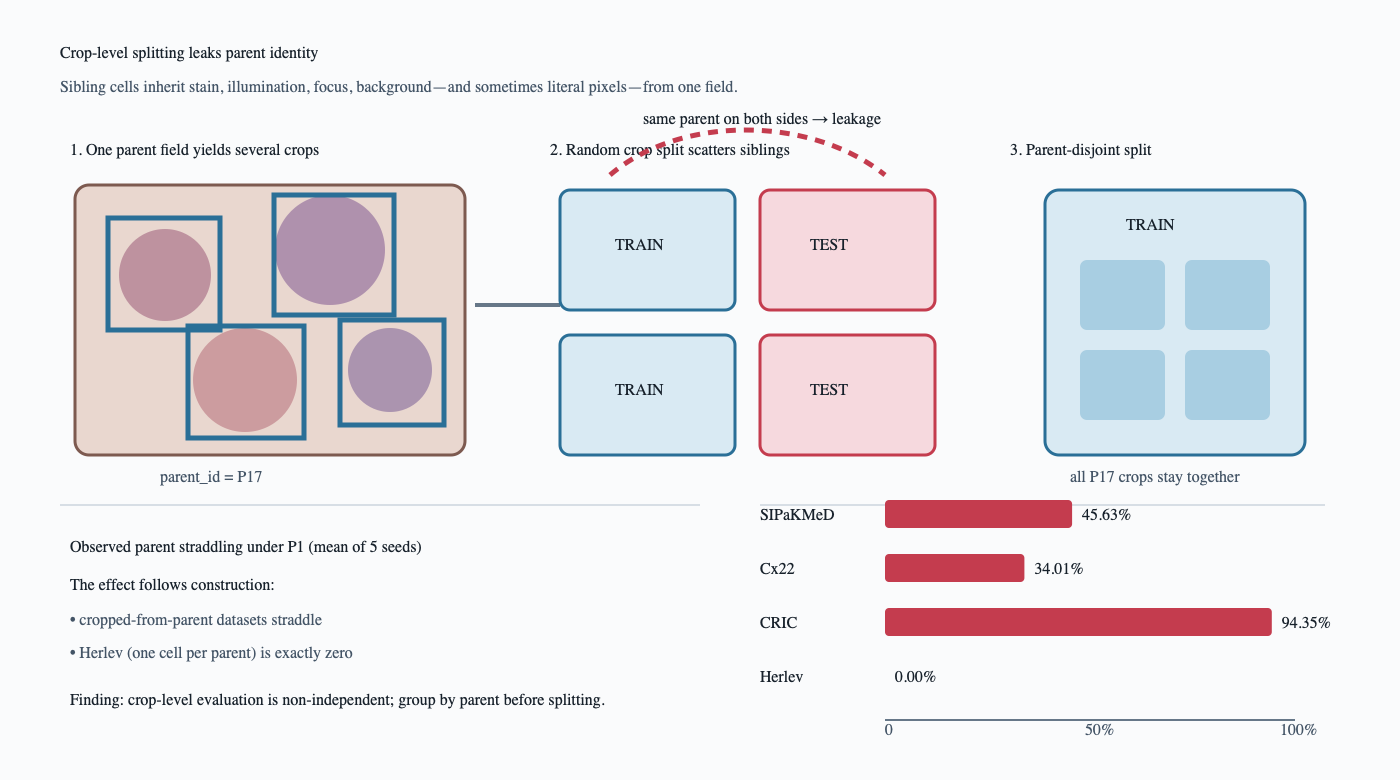
\includegraphics[width=\linewidth]{rendered/figure1.png}
\end{minipage}\hfill
\begin{minipage}[c]{0.25\textwidth}
\centering
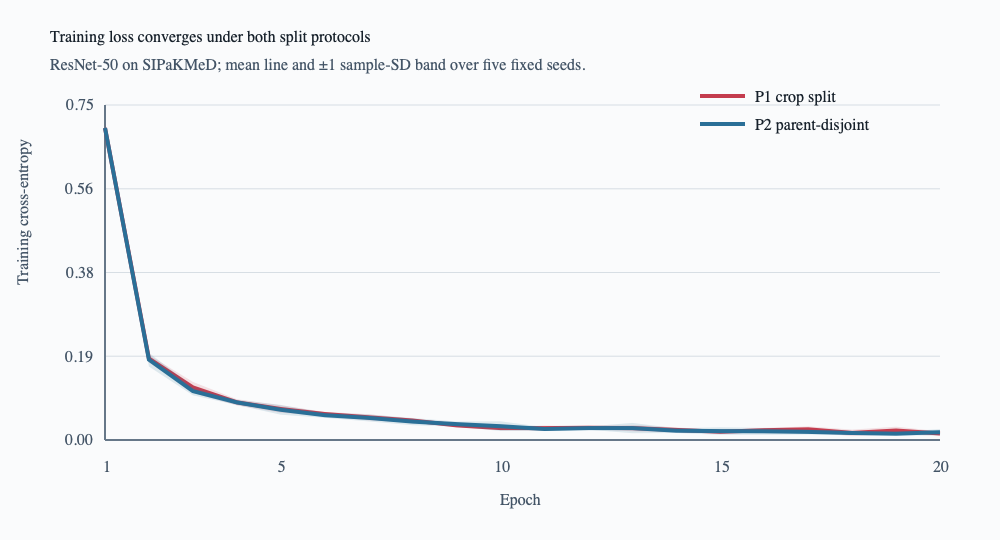
\includegraphics[width=\linewidth]{rendered/figure4.png}
\end{minipage}
\caption{Qualitative provenance and optimization diagnostics. Left: sibling crops can inherit a common field fingerprint, while parent grouping keeps them together. Right: frozen ResNet-50 training-loss histories converge under both split protocols.}
\label{fig:qualitative}
\end{figure*}

\section{Discussion}
The main finding is structural rather than architectural.
Random crop splitting makes the nominal test set extensively non-independent: most SIPaKMeD test crops have a training parent, more than half share literal source pixels with a training crop, and a model can identify the parent far above chance even from background-only inputs.
The same measurement correctly returns zero for the one-cell-per-parent Herlev structural negative control, while the high-crop-per-field CRIC construction produces the largest straddle rate.
These construction-linked results, dual-branch agreement, and analytic sanity check are mutually independent safeguards against a split-implementation artifact.

The two weakest architecture--protocol cells are MobileNet-V2 under \protocol{P2} (\meanpm{95.16}{1.50}\%) and ViT-B/16 under \protocol{P3} (\meanpm{95.53}{1.68}\%).
Their interpretation must remain aggregate because a class confusion matrix is unavailable in the frozen evidence.
Two real dataset properties nevertheless explain why grouped test composition can be unstable without claiming a particular error pair: crop counts are nearly balanced (787--831 per class), whereas parent counts range from 108 Parabasal fields to 271 Metaplastic fields, and cervical categories are defined by related morphological characteristics rather than separated acquisition domains.
Thus a parent-disjoint fold can preserve crop totals while changing the diversity of independently sourced appearances.
The larger ViT-B/16 \protocol{P3} SD is consistent with such composition sensitivity, but is not proof of a class-specific mechanism.

All six \protocol{P1}$-$\protocol{P2} estimates are positive, yet none survives the declared BH family, and four architectures violate the registered \protocol{P3}$\leq$\protocol{P2}$\leq$\protocol{P1} prediction.
We therefore do not claim universal accuracy inflation or causal shortcut use.
The justified conclusion is narrower: the crop is not the independent sampling unit, the source signal is available to a learner, and \protocol{P2} removes the measured parent and pixel sharing while preserving the same SIPaKMeD crop counts.

\section{Limitations}
The audited public datasets are modest in independent-parent count, and only SIPaKMeD received the complete six-architecture rescore, limiting claims about the magnitude of downstream performance changes.
No prospective clinical validation, patient-level outcome study, or deployment analysis was performed, so the corrected benchmark scores must not be read as estimates of clinical utility.
Training was constrained to at most three RTX A6000 GPUs, which limited broader full-matrix reruns, and the frozen aggregate run artifacts cannot support a post-hoc class confusion matrix without violating the hard stop.

\section{Conclusion}
We investigated whether public cervical-cytology classifiers were evaluated on genuinely independent cells and found that crop filenames concealed a consequential source-field hierarchy.
\cytofair{} recovered exact provenance, validated the reconstruction independently, measured parent straddling and literal pixel sharing, demonstrated a learnable parent-field fingerprint, and produced fixed parent-disjoint splits.
On SIPaKMeD, most crop-level test observations had a parent in training and more than half shared source pixels with a training crop; Cx22 and CRIC showed the same structural pattern, while Herlev behaved as the expected zero-leakage control.
Across six classifiers, ordinary crop splitting yielded positive \protocol{P1}$-$\protocol{P2} point estimates for every architecture, but the preregistered multiplicity-corrected evidence did not establish a universal accuracy-inflation effect.
The failed monotonic \protocol{P3} prediction was retained and narrowed the claim further: provenance-aware grouping corrects the evaluation unit, but a more conservative group definition need not monotonically reduce finite-sample accuracy.
The resulting contribution was therefore a benchmark correction and reusable measurement resource rather than another incremental classifier.
In V2, we will preregister a provenance-aware instance-segmentation evaluation on Cx22 and extend the same grouping apparatus to specimen-disjoint multi-view Fish-Pak and temporally grouped Croatian Fish video, with deterministic manifests fixed before model training.

\bibliographystyle{IEEEtran}
{\scriptsize\bibliography{references}}

\end{document}
